\documentclass[9pt,twocolumn,twoside,lineno]{pnas-new}
% Use the lineno option to display guide line numbers if required.
% Note that the use of elements such as single-column equations
% may affect the guide line number alignment. 

\templatetype{pnasresearcharticle} % Choose template 
% {pnasresearcharticle} = Template for a two-column research article
% {pnasmathematics} = Template for a one-column mathematics article
% {pnasinvited} = Template for a PNAS invited submission

\usepackage{units}
\usepackage{subfig}
\newtheorem{remark}{Remark}


\title{A Statistical Dynamical Model to Predict Extreme Events and Anomalous Features in Shallow Water Waves with Abrupt Depth Change}

% Use letters for affiliations, numbers to show equal authorship (if applicable) and to indicate the corresponding author
\author[a,1]{Andrew J. Majda}
\author[b]{M. N. J. Moore}
\author[a,1]{Di Qi} 


\affil[a]{Department of Mathematics and Center for Atmosphere
and Ocean Science, Courant Institute of Mathematical Sciences, New
York University, New York, NY 10012}
\affil[b]{Department of Mathematics and Geophysical Fluid
Dynamics Institute, Florida State University, Tallahassee, FL}


% Please give the surname of the lead author for the running footer
\leadauthor{Majda} 

% Please add here a significance statement to explain the relevance of your work
\significancestatement{Understanding and predicting extreme events and their anomalous statistics in complex nonlinear systems is a grand challenge in applied sciences as well as for engineering design. Recent controlled
laboratory experiments in weakly turbulent shallow water with abrupt
depth change exhibit a remarkable transition from nearly Gaussian
statistics to  extreme anomalous statistics with large
positive skewness of the surface height. We develop a statistical
dynamical model to explain and quantitatively predict the anomalous
statistical behavior. The incoming and outgoing  wares are modeled by the truncated Korteweg-de Vries equations statistically matched at the depth change.
The statistical matching of the known nearly Gaussian incoming Gibbs
state completely determines the predicted anomalous outgoing
Gibbs state, and successfully captures key features
of the experiment.}

% Please include corresponding author, author contribution and author declaration information
\authorcontributions{A.J.M. designed the research. A.J.M., M.N.J.M., and D.Q. performed the research. A.J.M., M.N.J.M., and D.Q. wrote the paper.}
\authordeclaration{The authors declare no conflict of interest.}
%\equalauthors{\textsuperscript{1}A.J.M.(Author One) and D.Q. (Author Two) contributed equally to this work.}
\correspondingauthor{\textsuperscript{1}To whom correspondence should be addressed. E-mail: qidi@cims.nyu.edu, jonjon@cims.nyu.edu}

% Keywords are not mandatory, but authors are strongly encouraged to provide them. If provided, please include two to five keywords, separated by the pipe symbol, e.g:
\keywords{extreme anomalous event $|$ statistical TKdV model $|$ matching Gibbs measures $|$ surface wave displacement and slope} 

\begin{abstract}
Understanding and predicting extreme events and their anomalous statistics
in complex nonlinear systems is a grand challenge in climate, material,
and neuroscience, as well as for engineering design. Recent controlled
laboratory experiments in weakly turbulent shallow water with abrupt
depth change (ADC) exhibit a remarkable transition from nearly Gaussian
statistics in incoming wave trains before the ADC to outgoing waves
trains after the ADC with extreme anomalous statistics with large
positive skewness of the surface height. Here we develop a statistical
dynamical model to explain and quantitatively predict the above anomalous
statistical behavior as experimental control parameters are varied.
The first step is to use incoming and outgoing truncated Korteweg-de
Vries (TKdV) equations matched in time at the ADC. The TKdV equation
is a Hamiltonian system which induces incoming and outgoing statistical
Gibbs invariant measures which are statistically matched at the ADC.
The statistical matching of the known nearly Gaussian incoming Gibbs
state at the ADC completely determines the predicted anomalous outgoing
Gibbs state, which can be calculated by a simple sampling algorithm, verified
by direct numerical simulations, and successfully captures key features
of the experiment. There is even an analytic formula for the anomalous
outgoing skewness. The strategy here should be useful for predicting
extreme anomalous statistical behavior in other dispersive media in
different settings.
\end{abstract}

\dates{This manuscript was compiled on \today}
\doi{\url{www.pnas.org/cgi/doi/10.1073/pnas.XXXXXXXXXX}}

\begin{document}

% Optional adjustment to line up main text (after abstract) of first page with line numbers, when using both lineno and twocolumn options.
% You should only change this length when you've finalised the article contents.
\verticaladjustment{-2pt}

\maketitle
\thispagestyle{firststyle}
\ifthenelse{\boolean{shortarticle}}{\ifthenelse{\boolean{singlecolumn}}{\abscontentformatted}{\abscontent}}{}

% If your first paragraph (i.e. with the \dropcap) contains a list environment (quote, quotation, theorem, definition, enumerate, itemize...), the line after the list may have some extra indentation. If this is the case, add \parshape=0 to the end of the list environment.
\dropcap{U}nderstanding and predicting extreme events and their anomalous statistics
in complex nonlinear systems is a grand challenge in climate, material
and neuroscience as well as for engineering design. This is a very
active contemporary topic in applied mathematics with qualitative
and quantitative models \cite{majda2012lessons,mohamad2018sequential,qi2016predicting,majda2015intermittency,majda2018model,majda2018simple,thual2016simple}
and novel numerical algorithms which overcome the curse of dimension
for extreme event prediction in large complex systems \cite{chen2018efficient,chen2017beating,chen2018conditional,mohamad2018sequential,qi2018predicting}.
The occurrence of Rogue waves as extreme events with different physical
settings of deep water \cite{adcock2014physics,cousins2015unsteady,farazmand2017reduced,onorato2001freak,dematteis2018rogue}
and shallow water \cite{sergeeva2011nonlinear,trulsen2012laboratory,viotti2014extreme}
is an important practical topic.

Recent controlled laboratory experiments in weakly turbulent shallow
water with abrupt depth change (ADC) exhibit a remarkable transition
from nearly Gaussian statistics in incoming wave trains before the
ADC to outgoing waves trains after the ADC with extreme anomalous
statistics with large positive skewness of the surface height \cite{bolles2018anomalous}.
Here we develop a statistical dynamical model to explain and quantitatively
predict the above anomalous statistical behavior as experimental control
parameters are varied. The first step is to use incoming and outgoing
truncated Korteweg-de Vries (TKdV) equations matched in time at the
ADC. The TKdV equation is a Hamiltonian system which induces incoming
and outgoing statistical Gibbs invariant measures which are statistically
matched at the ADC. The statistical matching of the known nearly Gaussian
incoming Gibbs state at the ADC completely determines the predicted
anomalous outgoing Gibbs state, which can be calculated by a simple
MCMC algorithm, verified by direct numerical simulations, and successfully
captures key features of the experiment. There is even an analytic
formula for the anomalous outgoing skewness. The strategy here should
be useful for predicting extreme anomalous statistical behavior in
other dispersive media in different settings.

\section{Experiments showing anomalous wave statistics by the abrupt depth change}

A series of experiments are carried out \cite{bolles2018anomalous}
studying the anomalous statistical behaviors in surface water waves
going through an abrupt depth transition. The unidirectional waves
propagate along a water tank over a step in the bottom topography,
and the surface displacements of the wave levels are measured at several
upstream and downstream locations. The wave field is excited by a
paddle wheel forcing with angle
\[
\theta\left(t\right)=\theta_{0}+\Delta\theta\sum_{n=1}^{N}a_{n}\cos\left(\omega_{n}t+\delta_{n}\right),\;E\sim\left(\Delta\theta\right)^{2}\sum_{n}a_{n}^{2}\omega_{n}^{2}.
\]
The total energy $E$ in the system is determined by the angle amplitude
$\Delta\theta$. Several observations are found in the anomalous wave
statistics:
\begin{itemize}
\item Distinct statistics are found between the incoming and outgoing wave
disturbances: the incoming waves display near-Gaussian statistics,
while the outgoing waves show skewness toward the positive displacement.
\item The non-Gaussian statistics is related with the total energy contained
in the system: larger driving amplitude $\Delta\theta$ will generate
stronger skewness in the PDFs.
\item The waves also show different characteristic peak wavelengths in incoming
and outgoing flows.
\end{itemize}

\section{Surface wave turbulence modeled by truncated KdV equation with depth dependence\label{sec:Surface-wave-turbulence}}

The surface wave turbulence is modeled by a one-dimensional deterministic
dynamical model. The Korteweg-de Vries (KdV) equation \cite{johnson1997modern}
is a leading-order approximation of the surface waves that are determined
by the balance of nonlinear and dispersive effects in an appropriate
far-field limit. Here, the KdV equation is truncated in the first
$\Lambda$ modes (with $J=2\Lambda+1$ grid points) to generate weakly
turbulent dynamics. Therefore, the surface disturbance is modeled by
the state variable $u_{\Lambda}^{\pm}\left(x,t\right)$ with superscript `$-$'
for the incoming waves and `$+$' for the outgoing waves. The Galerkin
truncated variable $u_{\Lambda}=\sum_{1\leq\left|k\right|\leq\Lambda}\hat{u}_{k}\left(t\right)e^{ikx}$
is normalized with zero mean $\hat{u}_{0}=0$ and unit energy $2\pi\sum_{k=1}^{\Lambda}\left|\hat{u}_{k}\right|^{2}=1$,
which are conserved quantities, and $u_{\Lambda}\equiv\mathcal{P}_{\Lambda}u$
denotes the subspace projection. The motion is governed by the truncated
KdV equation with depth change $D_{\pm}$ about the state variable
$u_{\Lambda}^{\pm}$
\begin{equation}
\frac{\partial u_{\Lambda}^{\pm}}{\partial t}+\frac{D_{\pm}^{-3/2}}{2}E_{0}^{1/2}L_{0}^{-3/2}\frac{\partial}{\partial x}\mathcal{P}_{\Lambda}\left(u_{\Lambda}^{\pm}\right)^{2}+D_{\pm}^{1/2}L_{0}^{-3}\frac{\partial^{3}u_{\Lambda}^{\pm}}{\partial x^{3}}=0,\label{eq:tKdV_nondim}
\end{equation}
on the normalized periodic domain $x\in\left[-\pi,\pi\right]$ with the conserved Hamiltonian decomposed into the difference of two
components containing the cubic and quadratic terms
\begin{align*}
\mathcal{H}_{\Lambda}^{\pm} & =  D_{\pm}^{-3/2}E_{0}^{1/2}L_{0}^{-3/2}H_{3}\left(u_{\Lambda}^{\pm}\right)-D_{\pm}^{1/2}L_{0}^{-3}H_{2}\left(u_{\Lambda}^{\pm}\right),\\
& H_{3}\left(u\right) =  \frac{1}{6}\int_{-\pi}^{\pi}u^{3}dx,\;H_{2}\left(u\right)=\frac{1}{2}\int_{-\pi}^{\pi}\left(\frac{\partial u}{\partial x}\right)^{2}dx.
\end{align*}
The model [\ref{eq:tKdV_nondim}] is non-dimensionalized in the periodic
domain. The depth is assumed to be unit $D_{-}=1$
before the abrupt depth change and becomes $D_{+}<1$ for the flows
after the change. We introduce the model parameters $\left(E_{0},L_{0},\Lambda\right)$
based on the following model assumptions:
\begin{itemize}
\item The wavenumber truncation $\Lambda$ is fixed in a moderate value
for generating weakly turbulent dynamics;
\item The state variable $u_{\Lambda}^{\pm}$ is normalized with zero mean
and unit energy, $\mathcal{M}\left(u_{\Lambda}\right)=0,\mathcal{E}\left(u_{\Lambda}\right)=1$,
conserved during the evolution, while $E_{0}$ characterizes the total
energy injected in the system based on the paddle amplitude $\left(\Delta\theta\right)^{2}$;
\item The length scale of the system is defined by $L_{0}$. The value is
chosen so that the resolved scale $\Delta x=2\pi L_{0}/J$ is comparable
with the the characteristic wave length $\lambda_{c}$ found from
the experiments.
\end{itemize}
The intuition for the distinct model dynamics comes from the balance
between the cubic and quadratic terms in the Hamiltonian $\mathcal{H}_{\Lambda}^{\pm}$.
After the depth change, $D_{+}<1$, more weight is added in the cubic
term, $H_{3}$, for stronger nonlinearity and weaker dispersion for
the third-order derivative term reflected by the smaller coefficient
for $H_{2}$ in the Hamiltonian. Since $\frac{\partial u}{\partial x}$
is the slope of the wave height, $H_{2}\left(u\right)$ measures the
wave slope energy.

A \emph{deterministic matching condition} is given for the surface
displacement $u_{\Lambda}^{\pm}$ agreeing at the locations before
and after the abrupt depth change $T_{\mathrm{ADC}}$
\[
u_{\Lambda}^{-}\left(x,t\right)\mid_{t=T_{\mathrm{ADC}}-}=u_{\Lambda}^{+}\left(x,t\right)\mid_{t=T_{\mathrm{ADC}}+},
\]
assuming the abrupt depth change is met at $t=T_{\mathrm{ADC}}$.
Equation [\ref{eq:tKdV_nondim}] is not designed to capture the short
scale changes in rapid time. On the other hand, we are interested
in the model statistical transition before and after the depth change,
so it is reasonable to observe the suitable slow-time performance
in the large scale structures.

\subsection{Interpreting experimental parameters in the dynamical model}

The model parameters $\left(E_{0},L_{0},\Lambda\right)$ in [\ref{eq:tKdV_nondim}]
can be directly linked with the basic scales from the physical problem.
The important characterizing parameters measured from the experiments
include: $\epsilon=\frac{a}{H_{0}}$ the wave amplitude $a$ to water
depth $H_{0}$ ratio; $\delta=\frac{H_{0}}{\lambda_{c}}$ the water
depth to wavelength scale $\lambda_{c}$ ratio; and $D_{0}=\frac{d}{H_{0}}$
the normalized wave depth ratio with incoming flow depth $d=H_{0}$
to the outgoing flow depth $d<H_{0}$. The interpretations and reference
values of these model parameters are based on the experimental setup
\cite{bolles2018anomalous}. By comparing the characteristic physical
scales, the normalized TKdV equation [\ref{eq:tKdV_nondim}] can be
linked directly with the measured non-dimensional quantities by
\begin{equation}
L_{0}=6^{\frac{1}{3}}\left(M\epsilon^{\frac{1}{2}}\delta^{-1}\right),\;E_{0}=\frac{27}{2}\gamma^{-2}\left(M\epsilon^{\frac{1}{2}}\delta^{-1}\right),\label{eq:params}
\end{equation}
where $M$ defines the computational domain size $L_{d}=M\lambda_{c}$
as $M$-multiple of the characteristic wavelength $\lambda_{c}$,
and $\gamma=\frac{U}{a}$ represents the factor to normalize the total
energy in the state variable $u_{\Lambda}$ to one. 

Consider the spatial discretization $J=2\Lambda+1$ so that the smallest
resolved scale is comparable with the characteristic wavelength
\[
\Delta x=\frac{2\pi M\lambda_{c}}{J}\lesssim\lambda_{c}\:\Rightarrow\:M=\frac{J}{2\pi}\sim5,\;J=32.
\]
Therefore in the practical numerical simulations, we pick $M=5$ and
$\gamma$ varies in the range $\left[0.5,1\right]$. Using the reference
experimental measurements \cite{bolles2018anomalous}, $\epsilon\in\left[0.0024,0.024\right],\delta\sim0.22$,
and $D_{0}$ changes from 1 to 0.24 before and after the depth change.
The reference values for the model scales can be estimated in the
range $L_{0}\in\left[2,6\right]$ and $E_{0}\in\left[50,200\right]$.
These are the values we will test in the direct numerical simulations.
See details about the derivation from scale analysis in \textcolor{blue}{\emph{SI Appendix, A}}.

\section{Equilibrium statistical mechanism for generating the stationary invariant measure}

Since the TKdV equation satisfies the Liouville property, the equilibrium
invariant measure can be described by an equilibrium statistical formulism
\cite{abramov2003hamiltonian,majda2006nonlinear,bajars2013weakly}
using a Gibbs measure with the conserved energy $\mathcal{E}_{\Lambda}$ and
Hamiltonian $\mathcal{H}_{\Lambda}$. The equilibrium invariant measure is dictated
by the conservation laws in the TKdV equation. In the case with fixed
total energy $E_{0}$, this is the \emph{mixed Gibbs measure} in the
truncated model with microcanonical energy and canonical Hamiltonian
ensembles \cite{abramov2003hamiltonian}
\begin{equation}
\mathcal{G}_{\theta}^{\pm}\left(u_{\Lambda}^{\pm};E_{0}\right)=C_{\theta}^{\pm}\exp\left(-\theta^{\pm}\mathcal{H}\left(u_{\Lambda}^{\pm}\right)\right)\delta\left(\mathcal{E}\left(u_{\Lambda}^{\pm}\right)-E_{0}\right),\label{eq:gibbs_mixed}
\end{equation}
with $\theta$ representing the ``inverse temperature''. The distinct
statistics in the upstream and downstream waves can be controlled
by the parameter value of the inverse temperature. The negative temperature
regime, $\theta^{\pm}<0$, is the appropriate regime to predict the
experiments as shown below. In the incoming flow field, the inverse
temperature $\theta^{-}$ is chosen so that $\mathcal{G}_{\theta}^{-}$
has Gaussian statistics. Using the above invariant measures [\ref{eq:gibbs_mixed}],
the expectation of any functional $F\left(u\right)$ can be computed
based on the Gibbs measure 
\[
\left\langle F\right\rangle _{\mathcal{G}_{\theta}}\equiv\int F\left(u\right)\mathcal{G}_{\theta}\left(u\right)du.
\]
The value of $\theta$ in the invariant measure is specified from
$\left\langle H_{\Lambda}\right\rangle _{\mathcal{G}_{\theta}}$ \cite{abramov2003hamiltonian,bajars2013weakly}.
The invariant measure also predicts an equilibrium energy spectrum
without running the TKdV equation directly. On the other hand, the
time autocorrelation and transient statistics about the state variable
$u_{\Lambda}$ cannot be recovered from the statistical theory.

\subsection{Statistical matching condition in invariant measures before and after the abrupt depth change}

The Gibbs measures $\mathcal{G}_{\theta}^{\pm}$ are defined based
on the different inverse temperatures $\theta^{\pm}$ on the two sides
of the solutions
\[
\begin{aligned}\mu_{t}^{-}\left(u_{\Lambda}^{-};D_{-}\right), & \quad u_{\Lambda}\mid_{t=T_{\mathrm{ADC}-}}=u_{0},\;t<T_{\mathrm{ADC}};\\
\mu_{t}^{+}\left(u_{\Lambda}^{+};D_{+}\right), & \quad u_{\Lambda}\mid_{t=T_{\mathrm{ADC}+}}=u_{0},\;t>T_{\mathrm{ADC}},
\end{aligned}
\]
where $u_{0}$ represents the deterministic matching condition between
the incoming and outgoing waves. The two distributions, $\mu_{t}^{-},\mu_{t}^{+}$
should also be matched at the depth change location $T_{\mathrm{ADC}}$,
so that
\[
\mu_{\infty}^{-}\left(u_{\Lambda}\right)=\mu_{t=T_{\mathrm{ADC}}}^{-}\left(u_{\Lambda}\right)=\mu_{t=T_{\mathrm{ADC}}}^{+}\left(u_{\Lambda}\right).
\]
In matching the flow statistics before and after the abrupt depth
change, first we use the conservation of the deterministic Hamiltonian
$H_{\Lambda}^{+}$ after the depth change. Then assuming ergodicity
\cite{abramov2003hamiltonian,majda2006nonlinear}, the statistical
expectation for the Hamiltonian $\left\langle H_{\Lambda}^{+}\right\rangle $
is conserved in time after the depth change at $t=T_{\mathrm{ADC}}$
and should stay in the same value as the system approaches equilibrium
as $t\rightarrow\infty$. The final statistical matching condition
to get the outgoing flow statistics with parameter $\theta^{+}$ can
be found by
\begin{equation}
\left\langle H_{\Lambda}^{+}\right\rangle _{\mathcal{G}_{\theta}^{+}}=\left\langle H_{\Lambda}^{+}\right\rangle _{\mathcal{G}_{\theta}^{-}},\label{eq:matching}
\end{equation}
with the outgoing flow Hamiltonian $H_{\Lambda}^{+}$ and the Gibbs
measures $\mathcal{G}_{\theta}^{\pm}$ before and after the abrupt
depth change.

\section{The nearly Gaussian incoming statistical state}

The incoming flow is always characterized by a near-Gaussian distribution
in the wave displacement. It is found that a physically consistent
Gibbs measure should take negative values in the inverse temperature
parameter $\theta<0$, where a proper distribution function and a
decaying energy spectrum are generated (see \cite{bajars2013weakly}
and \textcolor{blue}{\emph{SI Appendix, B.1}} for the explicit simulation results).
The upstream Gibbs measure $\mathcal{G}_{\theta}^{-}$ with $D_{-}=1$
displays a wide parameter regime in $\left(\theta^{-},E_{0}\right)$
with near-Gaussian statistics. In the left panel of Figure \ref{fig:matching}
(a), the inflow skewness $\kappa_3^{-}$ varies only within small amplitudes
among changing values of $E_{0}$ and $\theta^{-}$. The incoming
flow PDF then can be determined by picking the proper parameter value
$\theta^{-}$ in the near Gaussian regime with small skewness. In
contrast, the downstream Gibbs measure $\mathcal{G}_{\theta}^{+}$
with $D_{+}=0.24$ shown in the right panel of Figure \ref{fig:matching}
(a) generates much larger skewness $\kappa_3^{+}$ with highly skewed
PDFs as the absolute value of $\theta^{+}$ and the total energy level
$E_{0}$ increase in amplitude. The solid lines in Figure \ref{fig:matching}
(c) offer a further confirmation of the transition from near-Gaussian
statistics with tiny $\kappa_3^{-}$ to strongly skewed distribution
$\kappa_3^{+}$ after the depth change.

In the next step, the value of the downstream $\theta^{+}$ is determined
based on the matching condition [\ref{eq:matching}]. The expectation
$\left\langle H_{\Lambda}^{+}\right\rangle _{\mathcal{G}_{\theta}^{-}}$
about the incoming flow Gibbs measure can be calculated according
to the predetermined parameter values of $\theta^{-}$ as well as
$E_{0}$ from the previous step. For the direct numerical experiments
shown later in Figure \ref{fig:Changes-stats}, we pick proper choices
of test parameter values as $L_{0}=6, E_{0}=100$ and $\theta^{-}=-0.1,-0.3,-0.5$.
More test cases with different system energy $E_{0}$ can be found
in \textcolor{blue}{\emph{SI Appendix, B.2}} where similar transition from near
Gaussian symmetric PDFs to skewed PDFs in the flow state $u_{\Lambda}^{\pm}$
can always be observed.

\subsection{Direct numerical model simulations}

Besides the prediction of equilibrium statistical measures from the
equilibrium statistical approach, another way to predict the downstream
model statistics is through running the dynamical model [\ref{eq:tKdV_nondim}]
directly. The TKdV equation is found to be ergodic with proper mixing
property as measured by the decay of autocorrelations as long as the
system starts from a negative inverse temperature state as described
before. For direct numerical simulations of the TKdV equations, a
proper symplectic integrator is required to guarantee the Hamiltonian
and energy are conserved in time. It is crucial to use the symplectic
scheme to guarantee the exact conservation of the energy and Hamiltonian
since they are playing the central role in generating the invariant
measure and the statistical matching. The symplectic schemes used
here for the time integration of the equation is the 4th-order midpoint
method \cite{mclachlan1993symplectic}. Details about the mixing properties
from different initial states and the numerical algorithm are described
in \textcolor{blue}{\emph{SI Appendix, C}}.

\begin{figure}[h]
\centering
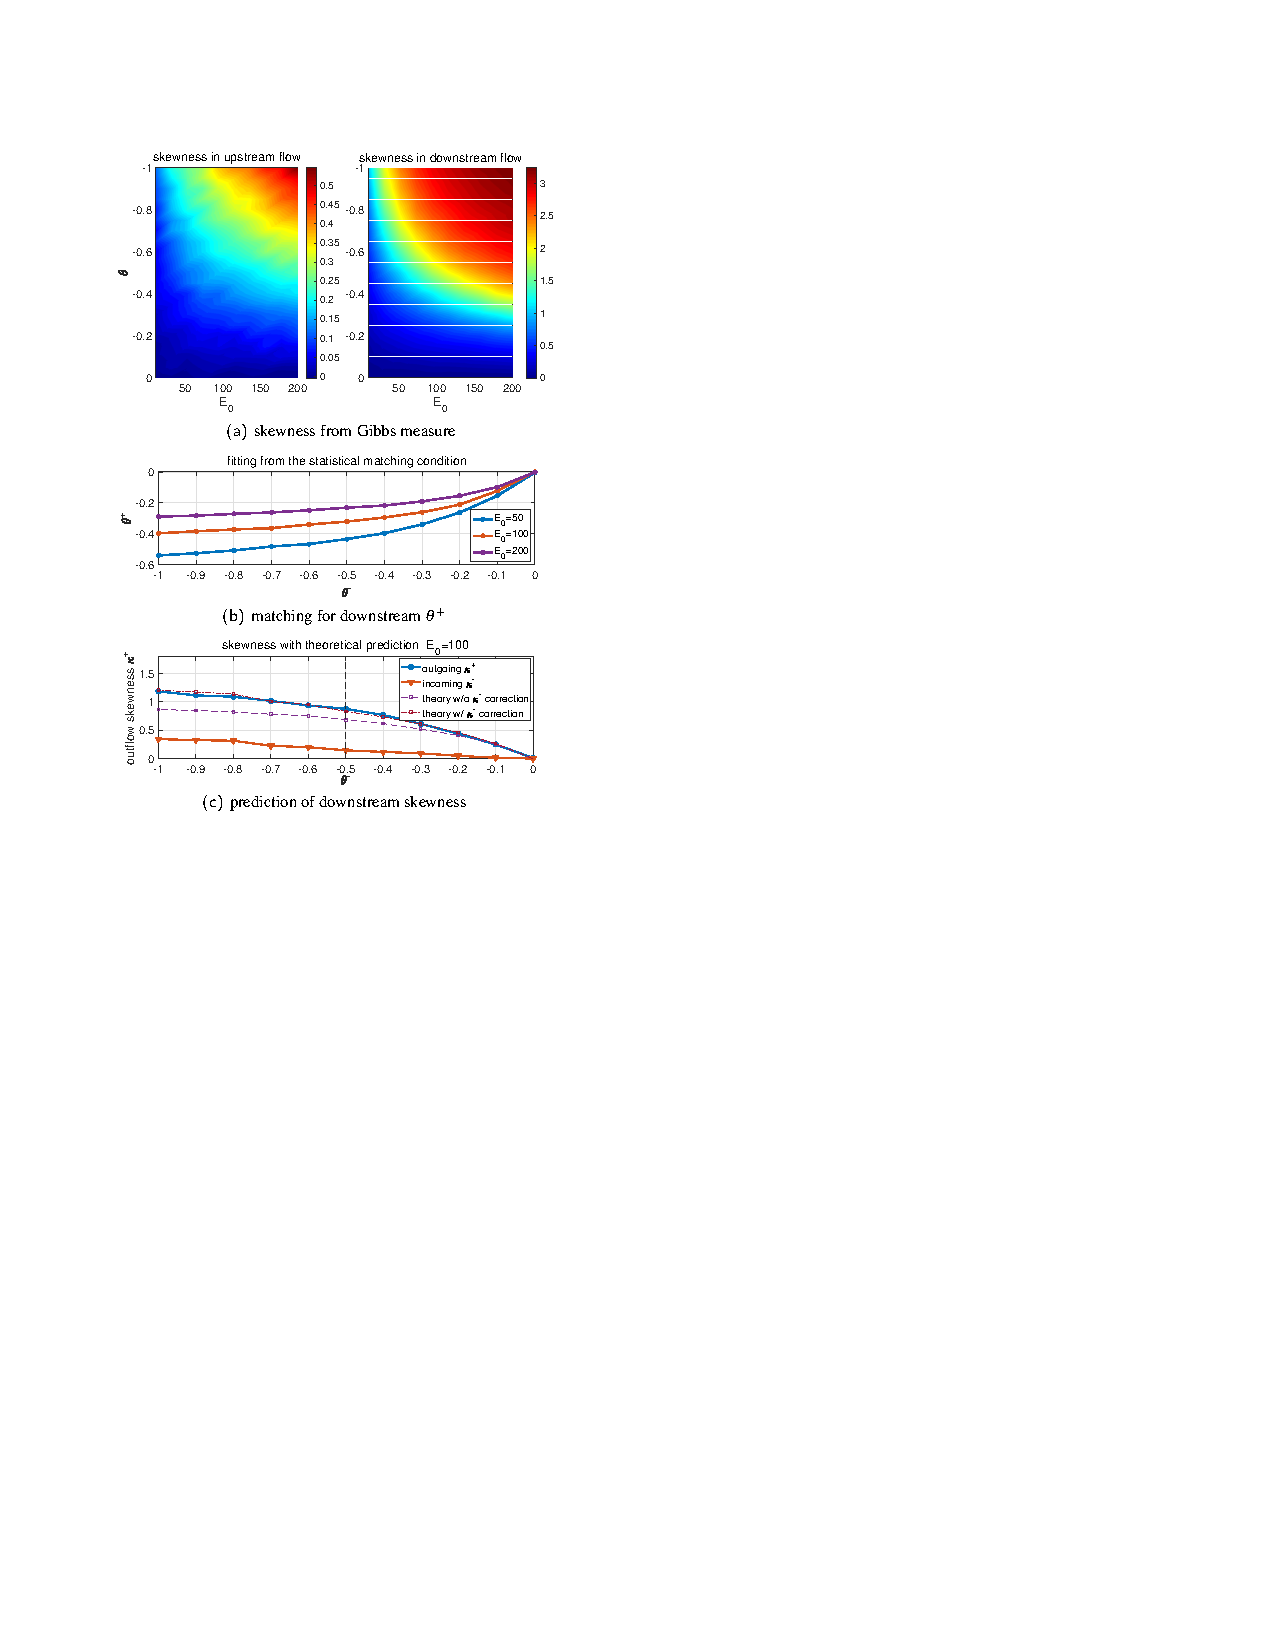
\includegraphics[scale=1.]{./fig1}

\caption{Fist row: skewness from the Gibbs measures in incoming and outgoing
flow states with different values of total energy $E_{0}$ and inverse
temperature $\theta$ (notice the different scales in the incoming
and outgoing flows); Second row: outgoing flow parameter $\theta^{+}$
as a function of the incoming flow $\theta^{-}$ computed from the
statistical matching condition with three energy level $E_{0}$; Last
row: skewness in the outgoing flow with the matched value of $\theta^{+}$
as a function of the inflow parameter $\theta^{-}$ (the theoretical
predictions using [\ref{eq:skewness}] are compared).\label{fig:matching}}
\end{figure}

\section{Predicting extreme anomalous behavior after the ADC by statistical matching}

With the inflow statistics well described and the numerical scheme
set up, we are able to predict the downstream anomalous statistics
starting from the near-Gaussian incoming flow going through the abrupt
depth change from $D_{-}=1$ to $D_{+}=0.24$. First, we consider
the statistical prediction in the downstream equilibrium measure directly
from the matching condition. The downstream parameter value $\theta^{+}$
is determined by solving the nonlinear equation [\ref{eq:matching}]
as a function of $\theta^{+}$, $F\left(\theta^{+}\right)=\left\langle H_{\Lambda}^{+}\right\rangle _{\mathcal{G}_{\theta}^{+}}\left(\theta^{+}\right)-\left\langle H_{\Lambda}^{+}\right\rangle _{\mathcal{G}_{\theta}^{-}}=0$.
In the numerical approach, we adopt a modified secant method avoiding
the stiffness in the parameter regime (see the \textcolor{blue}{\emph{SI Appendix, B.2}}
for the algorithm). The fitted solution is plotted in Figure
\ref{fig:matching} (b) as a function of the proposed inflow $\theta^{-}$.
A nonlinear $\theta^{-}$--$\theta^{+}$ relation is discovered from
the matching condition. The downstream inverse temperature $\theta^{+}$
will finally saturate at some level. The corresponding downstream
skewness of the wave displacement $u_{\Lambda}$ predicted from the
statistical matching of Gibbs measures is plotted in Figure \ref{fig:matching} (c). In general, a large positive skewness
for outgoing flow $\kappa_3^{+}$ is predicted from the theory, while
the incoming flow skewness $\kappa_3^{-}$ is kept in a small value
in a wide range of $\theta^{-}$. Note that with $\theta^{-}\sim0$
(that is, using the microcanonical ensemble only with energy conservation),
the outflow statistics are also near Gaussian with weak skewness.
The skewness in the outflow statistics grows as the inflow parameter
value $\theta^{-}$ increases in amplitude. 

For a second approach, we can use direct numerical simulations starting
from the initial state sampled from the incoming flow Gibbs measure
$\mathcal{G}_{\theta}^{-}$ and check the transient changes in the
model statistics. Figure \ref{fig:Changes-stats} illustrates the
change of statistics as the flow goes through the abrupt depth change.
The first row plots the changes in the skewness and kurtosis for the
state variable $u_{\Lambda}$ after the depth change at $t=0$. The
PDFs in the incoming and outgoing flow states are compared with three different
initial inverse temperatures $\theta^{-}$. After the depth changes
to $D_{0}=0.24$ abruptly at $t=0$, both the skewness and kurtosis
jump to a much larger value in a short time, implying the rapid transition
to a highly skewed non-Gaussian statistical regime after the depth
change. Further from Figure \ref{fig:Changes-stats}, different initial
skewness (but all relatively small) is set due to the various values
of $\theta^{-}$. With small $\theta^{-}=-0.1$, the change in the
skewness is not very obvious (see the second row of Figure \ref{fig:Changes-stats}
for the incoming and outgoing PDFs of $u_{\Lambda}$). In comparison,
if the incoming flow starts from the initial parameter $\theta^{-}=-0.3$
and $\theta^{-}=-0.5$, much larger increase in the skewness is induced
from the abrupt depth change. Furthermore, in the detailed plots in
the third row of Figure \ref{fig:Changes-stats} for the downstream PDFs
under logarithmic scale, fat tails towards the positive direction
can be observed, which represent the extreme events in the downstream
flow (see also Figure \ref{fig:Realization} for the time-series of
$u_{\Lambda}$).

As a result, the downstream statistics in final equilibrium predicted
from the direct numerical simulations here agree with the equilibrium
statistical mechanism prediction illustrated in Figure \ref{fig:matching}. The prediction from these two different approaches
confirm each other.

\begin{figure*}
\centering
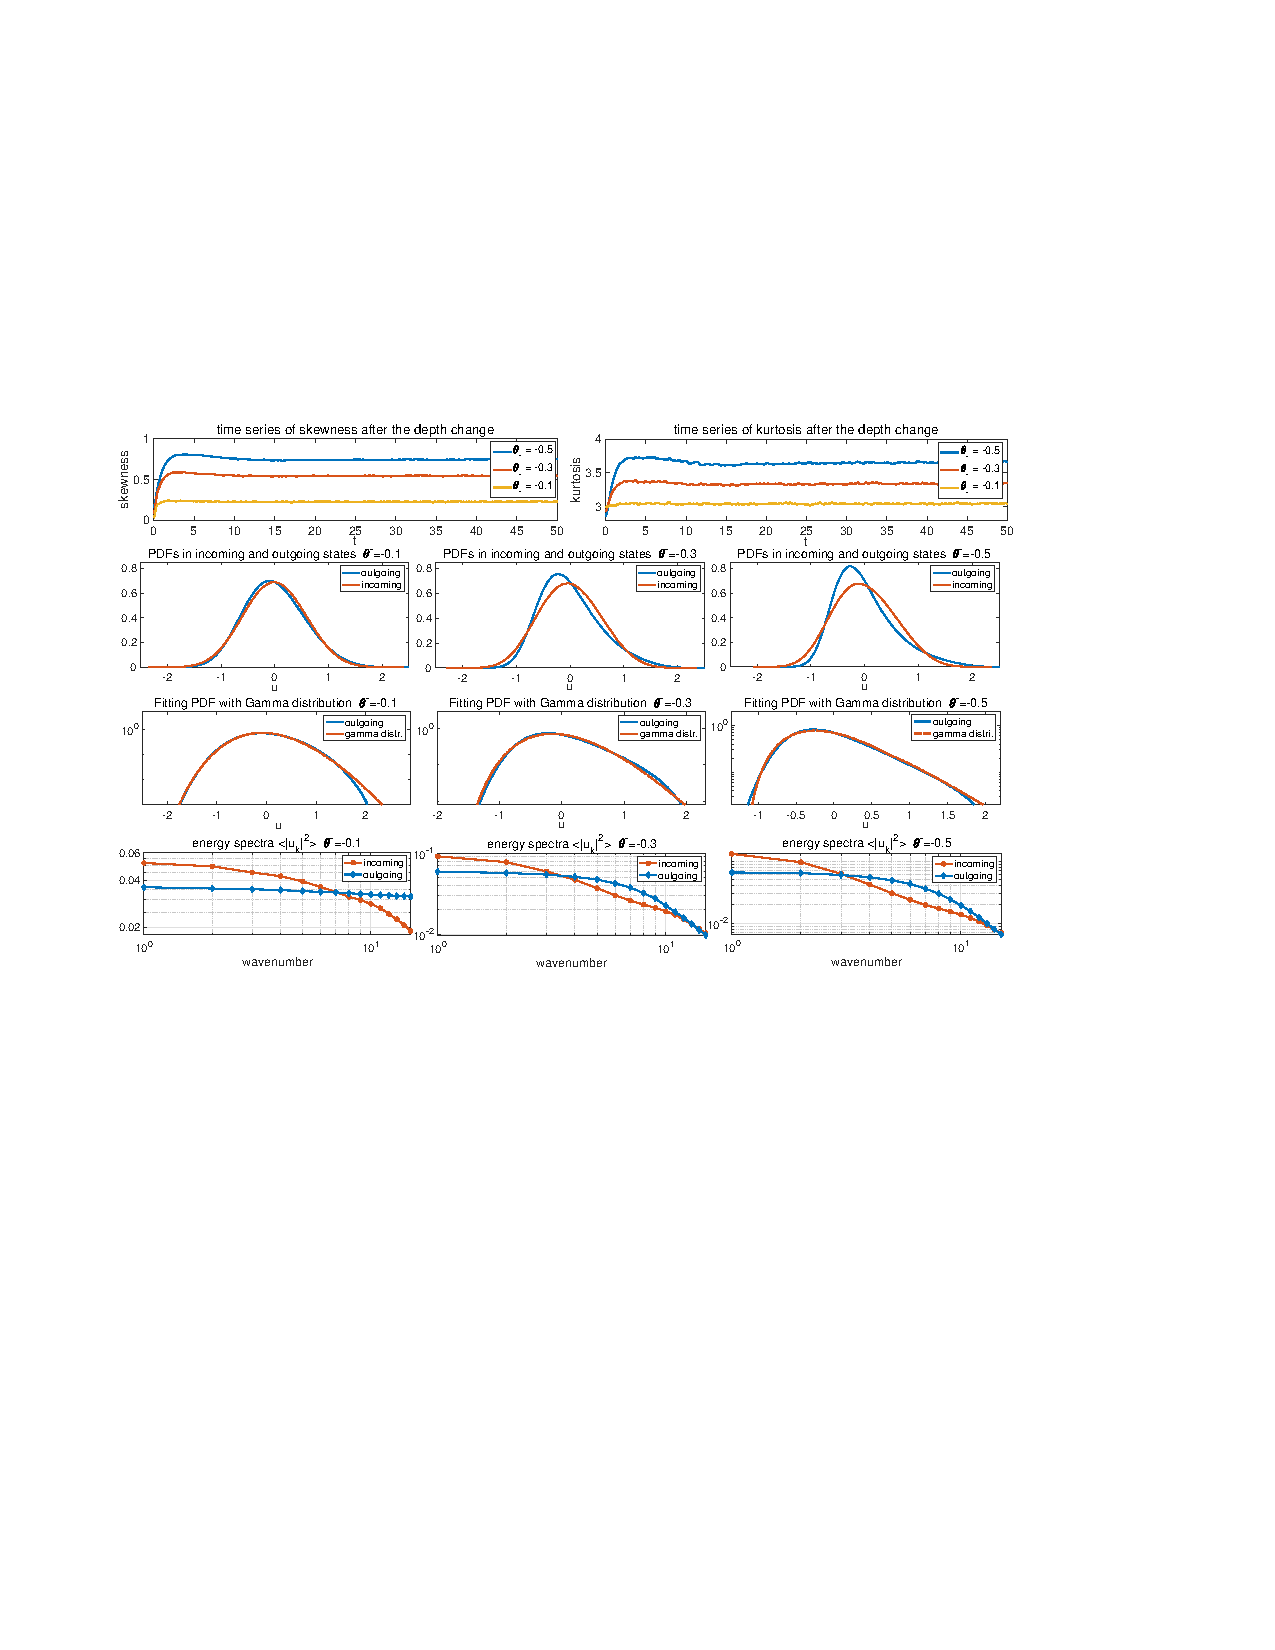
\includegraphics[scale=.9]{./fig2}

\caption{Changes in the statistics of the flow state going through the abrupt
depth change. The initial ensemble is set with the incoming flow Gibbs
measure with different inverse temperature $\theta^{-}$. First row:
time evolution of the skewness and kurtosis. The abrupt depth change
is taking place at $t=0$; Second row: inflow and outflow PDFs of
$u_{\Lambda}$; Third row: the downstream PDFs fitted with Gamma distributions
with consistent variance and skewness (in log coordinate in $y$);
Last row: energy spectra in the incoming and outgoing flows.\label{fig:Changes-stats}}
\end{figure*}

\section{Analytic formula for the upstream skewness after the ADC}

A statistical link between the upstream and downstream energy spectra
can be found for an analytical prediction of the skewness in the flow
state $u$ after the ADC. The skewness of the state variable $u_{j}$
at one spatial grid point is defined as the ratio between the third
and second moments
\[
\kappa_{3}=\left\langle u_{j}^{3}\right\rangle _{\mu}/\left\langle u_{j}^{2}\right\rangle _{\mu}^{\frac{3}{2}}.
\]
Now we introduce mild assumptions on the distribution functions:
\begin{itemize}
\item The upstream equilibrium measure $\mu_{-}$ has a relatively small
skewness so that
\[
\left\langle H_{3}\right\rangle _{\mu_{-}}=\frac{1}{6}\int_{-\pi}^{\pi}\left\langle u^{3}\right\rangle _{\mu_{-}}dx\equiv\epsilon;
\]
\item The downstream equilibrium measure $\mu_{+}$ is homogeneous at each
physical grid point, so that the second and third moments are invariant
at each grid point
\[
\left\langle u_{j}^{2}\right\rangle _{\mu_{+}}=\sigma^{2}=\pi^{-1},\quad\left\langle u_{j}^{3}\right\rangle _{\mu_{+}}=\sigma^{3}\kappa_{3}=\pi^{-\frac{3}{2}}\kappa_{3}^{+}.
\]
\end{itemize}
Then the skewness of the downstream state variable $u_{\Lambda}^{+}$
after the ADC is given by the difference between the inflow and outflow
wave slope energy of $u_x$
\begin{equation}
\begin{aligned}
\kappa_{3}^{+} = &\frac{3}{2}\pi^{\frac{1}{2}}L_{0}^{-\frac{3}{2}}E_{0}^{-\frac{1}{2}}D_{+}^{2}\int_{-\pi}^{\pi}\left[\left\langle u_{x}^{2}\right\rangle _{\mu+}-\left\langle u_{x}^{2}\right\rangle _{\mu-}\right]dx\\
 & +3\pi^{\frac{1}{2}}\epsilon.\label{eq:skewness}
\end{aligned}
\end{equation}
The detailed derivation is shown in \textcolor{blue}{\emph{SI Appendix, B.2}}.
In particular, the downstream skewness with near-Gaussian inflow statistics
$\epsilon\ll1$ is positive if and only if the difference of the incoming and outgoing 
wave slope energy is positive. This means that there is more
small scale wave slope energy in the outgoing state. As an evidence, 
in the last row of Figure \ref{fig:Changes-stats} in all the weak
and strong skewness cases, the outflow energy spectrum always has
a slower decay rate than the inflow energy spectrum which possesses
stronger energy in larger scales and weaker energy in the smaller
scales.

In Figure \ref{fig:matching} (c), we compare the accuracy of the
theoretical estimation [\ref{eq:skewness}] with numerical tests.
In the regime with small incoming inverse temperature $\theta^{-}$,
the theoretical formula offers a quite accurate approximation of the
third-order skewness using only information from the second-order
moments of the wave-slope spectrum. 

\section{Key features from experiments captured by the statistical dynamical model}

In this final section, we emphasize the crucial features generated
by the statistical dynamical model [\ref{eq:tKdV_nondim}] by making
comparison with the experimental observations in \cite{bolles2018anomalous}.
As from the scale analysis displayed in Section \ref{sec:Surface-wave-turbulence},
the theory is set in the same parameter regime as the experimental
setup.

\begin{figure*}[h]
\centering
\subfloat[downstream state $D_{0}=0.24$]{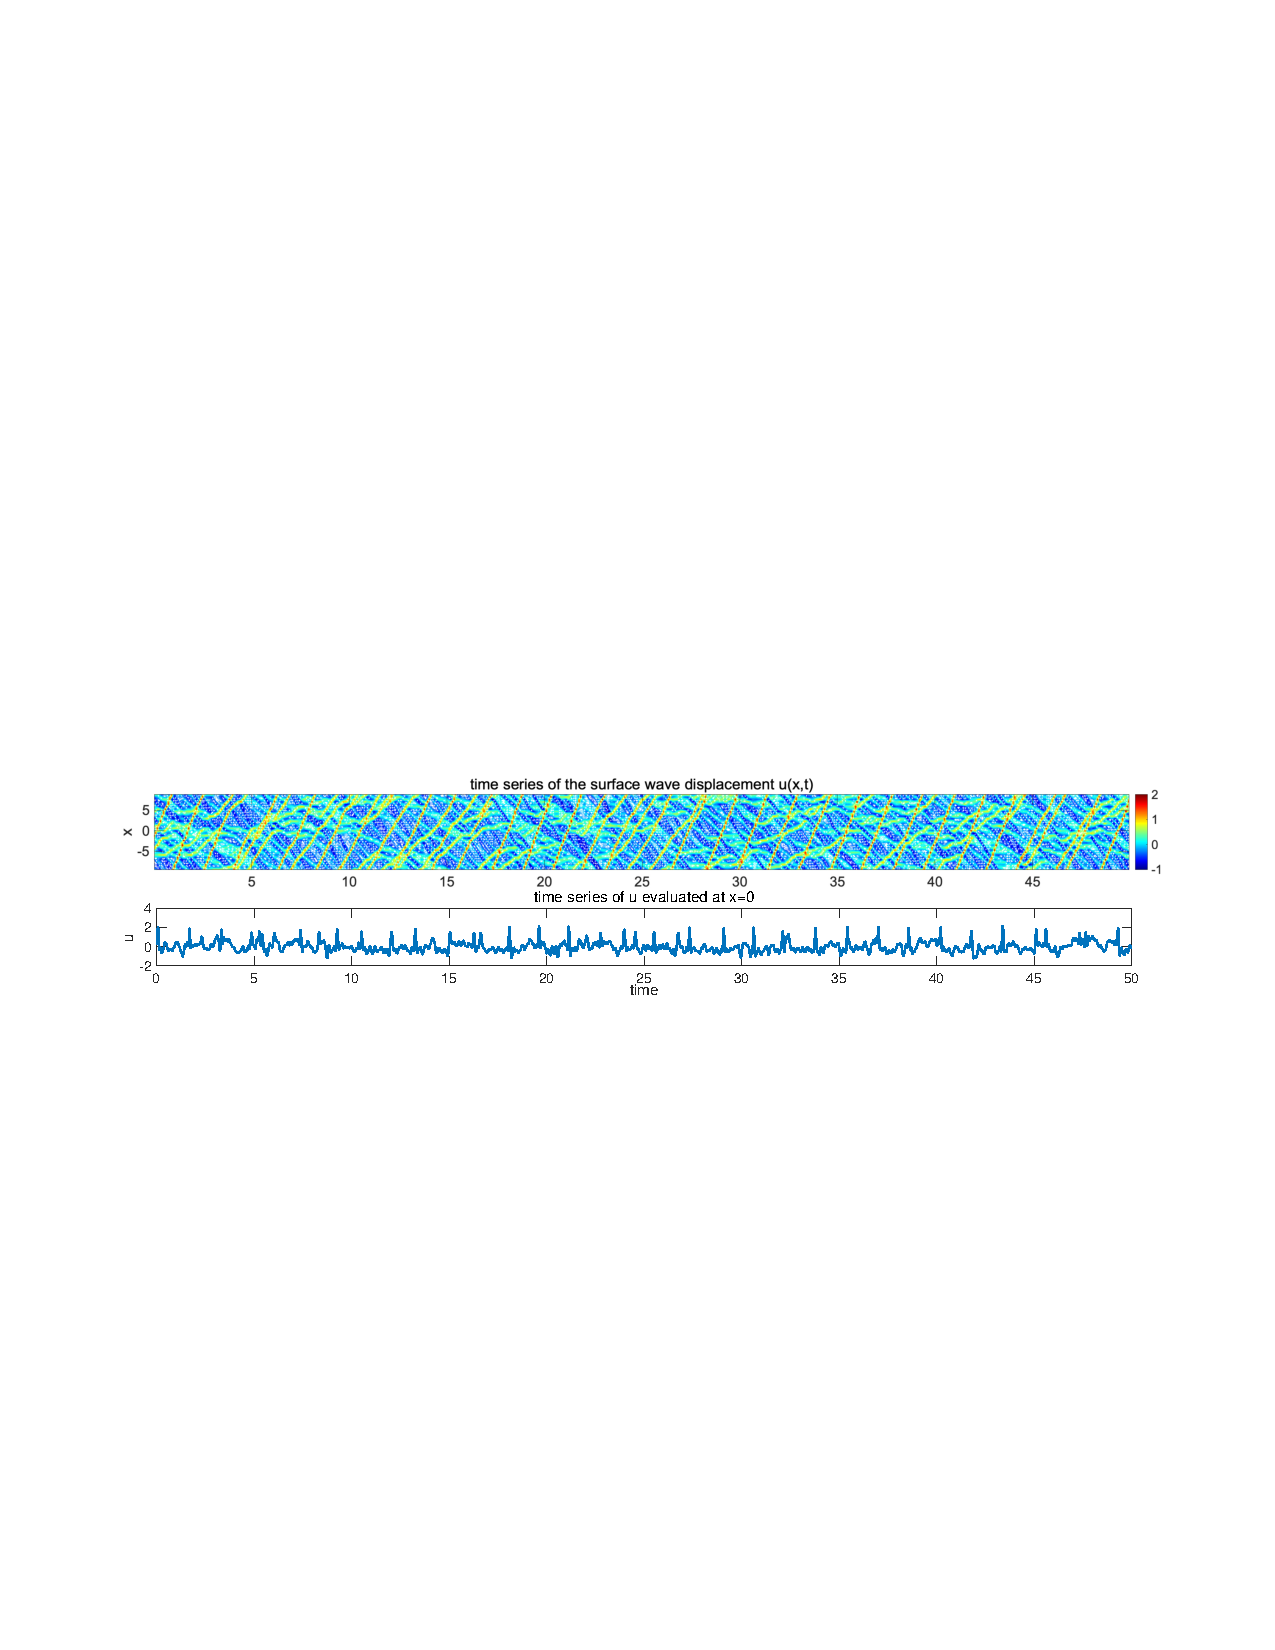
\includegraphics[scale=.95]{./fig3_1}}
\vspace{-1em}
\subfloat[upstream state $D_{0}=1$]{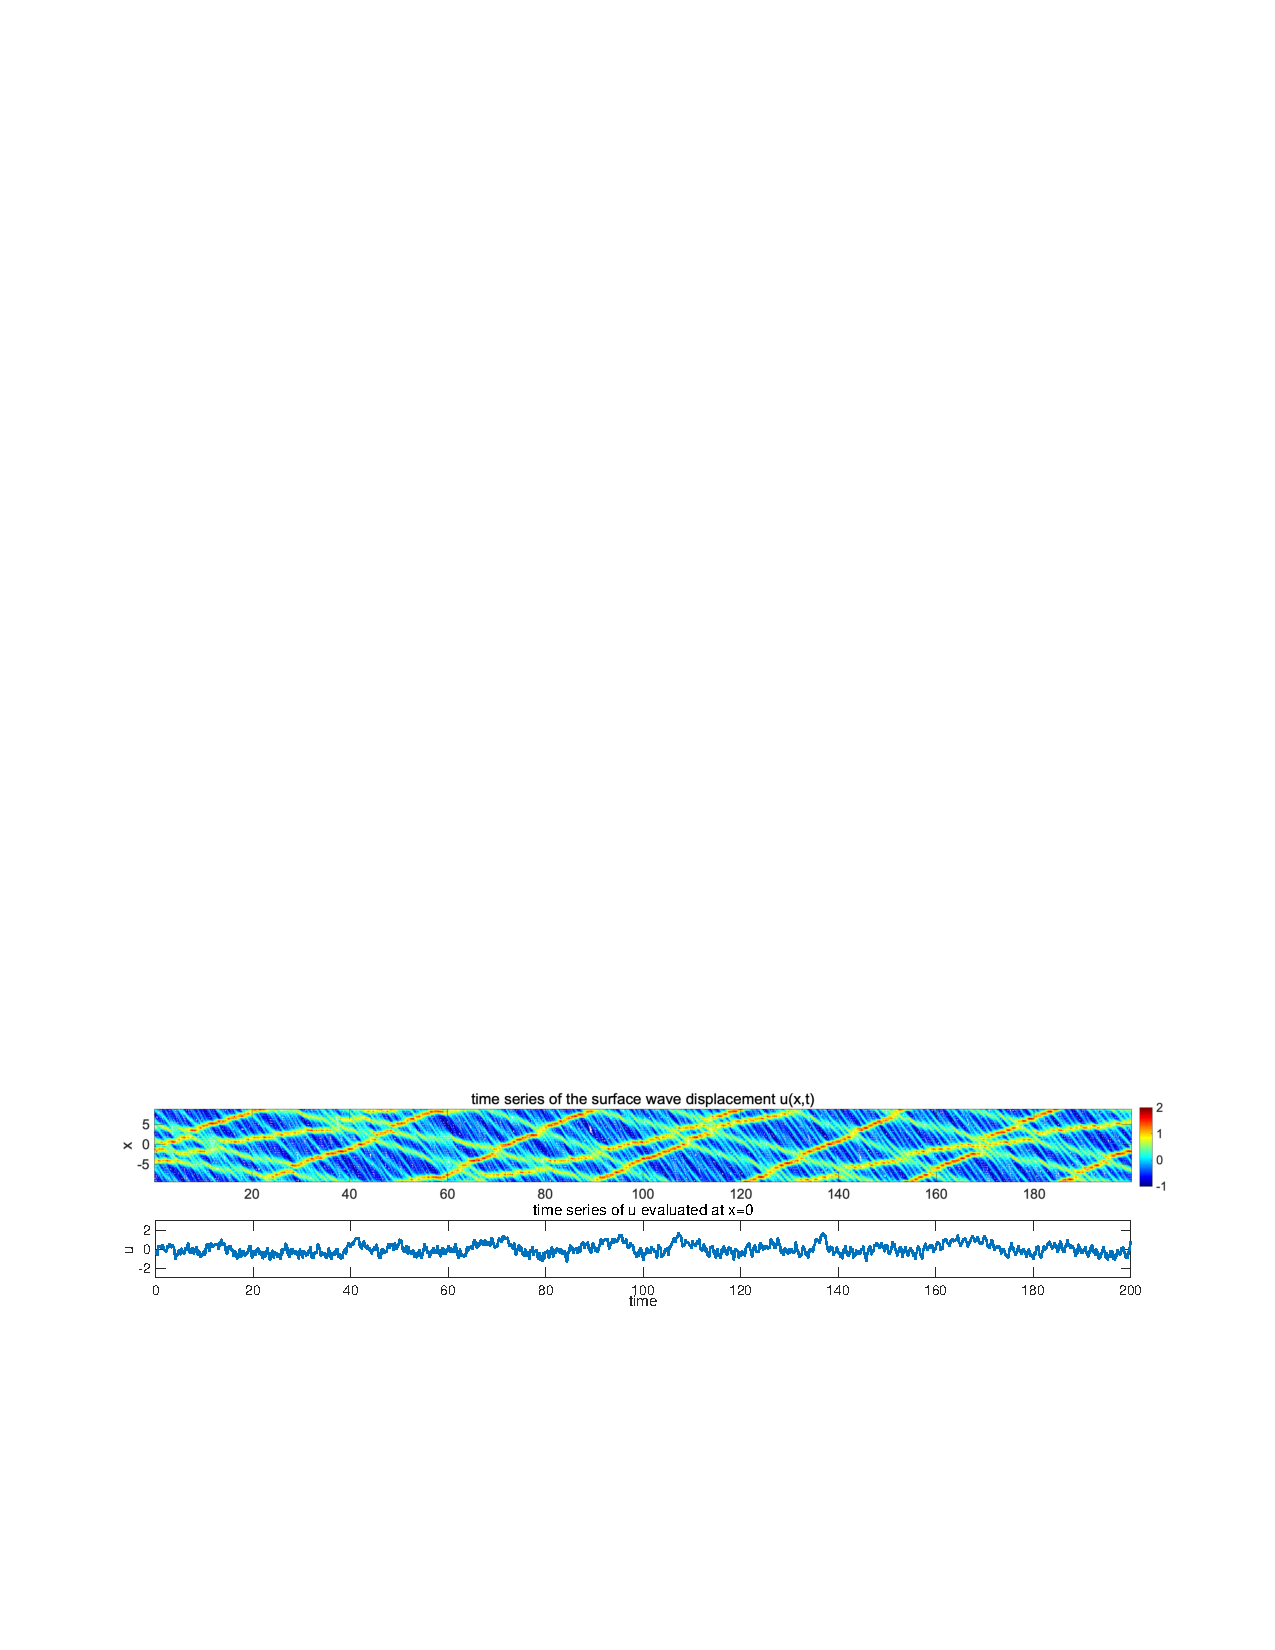
\includegraphics[scale=.95]{./fig3_2}}
\vspace{-1em}
\caption{Realization of the downstream and upstream flow solutions $u_{\Lambda}^{\pm}$. Note the larger vertical scale in the downstream time-series plot.\label{fig:Realization}}
\end{figure*}
\begin{itemize}
\item The transition from near-Gaussian to skewed non-Gaussian distribution
as well as the jump in both skewness and kurtosis observed in the
experiment observations (Fig. 1 of  \cite{bolles2018anomalous}) can
be characterized by the statistical model simulation results (see
the first and second row of Figure \ref{fig:Changes-stats}). Notice
that the difference in the decay of third and fourth moments in the far
end of the downstream regime from the experimental data is due to the
dissipation effect in the flow from the wave absorbers that is not modeled in the statistical
model here. The model simulation time-series plotted in Figure \ref{fig:Realization}
can be compared with the observed time sequences from experiments
(Fig. 1 of \cite{bolles2018anomalous}). The downstream simulation generates
waves with strong and frequent intermittency towards the positive
displacement, while the upstream waves show symmetric displacements
in two directions with at most small peaks in slow time. Even in the
time-series at a single location $x=0$, the long-time variation displays similar
structures. 
\item The downstream PDFs in experimental data are estimated with a Gamma
distribution in Fig. 2 of \cite{bolles2018anomalous}. Here in the same
way, we can fit the highly skewed outgoing flow PDFs from the numerical
results with the Gamma distribution
\[
\rho\left(u;k,\alpha\right)=\frac{e^{-k}\alpha^{-1}}{\Gamma\left(k\right)}\left(k+\alpha^{-1}u\right)^{k-1}e^{-\alpha^{-1}u}.
\]
The parameters $\left(k,\alpha\right)$ in the Gamma distribution
are fitted according to the measured statistics in skewness and variance,
that is, $\sigma^{2}=k\alpha^{2},\kappa_{3}=2/\sqrt{k}$. And the excess
kurtosis of the Gamma distribution can be recovered as $\kappa_{4}=6/k$.
As shown in the third row of Figure \ref{fig:Changes-stats}, excellent
agreement in the PDFs with the Gamma distributions
is reached in consistency with the experimental data observations.
The accuracy with this approximation increases as the initial inverse
temperature $\theta^{-}$ increases in value to generate more skewed
distribution functions.
\item The experiments also have the up and down stream power spectra in
time (Fig. 4 of \cite{bolles2018anomalous}), which shows more energy
at small time scales, i.e., a relatively slower decay rate in the
downstream compared with the upstream case. This is also observed
in the direct numerical simulations here (detailed results shown
in \textcolor{blue}{\emph{SI Appendix, C.2}}). The downstream state contains
more energetic high frequencies.
The peak frequency illustrates the occurrence of the transporting
waves along the water tank.
\end{itemize}

\section{Concluding discussion}

We have developed a statistical dynamical model to explain and predict
extreme events and anomalous features in shallow water waves with
abrupt depth change. The theory is based on the dynamical modeling
strategy consisting of the TKdV equation matched at the abrupt depth
change with conservation of energy and Hamiltonian. Predictions can
be made of the extreme events and anomalous features by matching incoming
and outgoing statistical Gibbs measures before and after the abrupt
depth transition. The statistical matching of the known nearly Gaussian
incoming Gibbs state completely determines the predicted anomalous
outgoing Gibbs state, which can be calculated by a simple sampling
algorithm, verified by direct numerical simulations, and successfully
captures key features of the experiment. An analytic formula for the
anomalous outgoing skewness is also derived. The strategy here should
be useful for predicting extreme statistical events in other dispersive
media in different settings.


\acknow{This research of A. J. M. is partially supported by the Office of
Naval Research through MURI N00014-16-1-2161. D. Q. is supported as
a postdoctoral fellow on the second grant. M.N.J.M }

\showacknow % Display the acknowledgments section

% \pnasbreak splits and balances the columns before the references.
% If you see unexpected formatting errors, try commenting out this line
% as it can run into problems with floats and footnotes on the final page.
\pnasbreak

% Bibliography
\bibliography{refs}

\end{document}